\documentclass[12pt,a4paper]{IEEEtran}

\usepackage[T1]{fontenc}
\usepackage[ngerman,english]{babel}
\usepackage[utf8]{inputenc}

\usepackage{standalone}

\usepackage[intlimits]{mathtools}
\usepackage{amsthm}
\usepackage{amssymb}
\usepackage{array}

\usepackage{tikz}
\usepackage{xcolor}
\usepackage{graphicx}
\usepackage{float}

\usepackage{tabularx}
\usepackage{multirow}
\usepackage{booktabs}

\usepackage[english]{isodate}
\usepackage[inline]{enumitem}
\usepackage{endnotes}
\renewcommand*{\enotesize}{\normalsize}
\let\oldenoteformat=\enoteformat
\renewcommand{\makeenmark}{\hbox{\(^{(\theenmark)}\)}}
\renewcommand{\enoteformat}{\noindent(\theenmark)\quad\llap}

\usepackage[autopunct]{csquotes}
\usepackage[natbib,backend=biber,bibencoding=inputenc,style=ieee]{biblatex}
\addbibresource{../references.bib}
\usepackage{hyperref}

\setlength{\parindent}{0pt}
\setlength{\parskip}{1ex}
\everymath{\displaystyle}

\DeclareMathOperator{\sgn}{sgn}
\newcommand{\osmattribute}[1][]{\mbox{#1 \textrm{\textcopyright} OpenStreetMap contributors}}
\newcommand{\n}{\ensuremath{-}}

\title{Inferring road network structure using link prediction}
\author{\IEEEauthorblockN{Ovidiu Victor T\u{a}tar}}
\date{\origdate\printdate{26.09.2020}}

\begin{document}

\maketitle

\begin{abstract}
This paper proposes a method for determining missing roads in a road-network using link prediction.
We load road-data from OpenStreetMap into Dgraph, a distributed graph database, and
use established similarity-functions as well as spacial information to determine
a link confidence for any given link.
For this task we train random forest classifiers and measure the accuracy of our predictions
on two similar datasets.
We find that the trained models produce at worst predictions with an average recall-rate over 16\%
while maintaining an average precision of at least 52\% and an overall average accuracy of over 99\%.
\end{abstract}

\IEEEpeerreviewmaketitle

\section{Introduction}

Infrastructure and by extension road networks have a significant impact on our
modern-day lives, as roads are an important part of transporting people and goods.
Gaining new insights into how road networks work and how they might change over time
can therefore be considered valuable information.
Traditionally this problem of analyzing networks over time and predicting changes has been approached using \emph{link prediction}.

Originally the problem of link prediction has been formalized for social networks~\cite[see][]{social_link_prediction},
but has since been applied to other fields.
Link prediction aims to find edges that are not included in a graph-dataset,
but are likely to be true and should be included in the dataset.~\cite[see][61]{knowledge_graphs}
The classical approach to link prediction popularized by \citeauthor{social_link_prediction} assigns a \emph{similarity score}
to every pair of nodes in a graph using a \emph{similarity function}.
These similarity scores can be used to determine the confidence of a given link existing in a graph-dataset.

Road networks can be expressed as graphs, therefore link prediction should be applicable to aid in the deduction of new information.
Possible applications include:
\begin{itemize}
\item generating realistic mock-up-data for other applications
\item reconstructing road networks with missing roads
      (for example a medieval road network, that was modernized and destroyed over the centuries)
\item predicting the evolution of a road network given its previous history; This could be helpful in city- and infrastructure-planning.
\item reimagining a road network in the style of another road network (\emph{style transfer} for road networks);
      This could be used for example to model how a rural area would evolve into a urban one
      or to aid in planning efficient road networks (by transferring knowledge about well designed road networks).
\end{itemize}
Each of these applications brings with them their own challenges,
we mention some of these as limitations in \autoref{sec:conclusion}.
Going forward we will not further explore these different applications in this paper,
instead they are a outlook for what we believe might be possible with future research.

This paper aims to apply link prediction to road networks and therefore to infer links (potential roads)
not present in a given road network.
Given a road network with incomplete data, the task is to predict how likely a link/road is
to connect two endpoints.
We propose utilizing established similarity-functions
as well as spacial information to train a random forest classifier to assign a
confidence for each given link.

\section{Related Work}\label{sec:related_work}

\citeauthor{road_link_prediction_subgraph} show problems of classical similarity-functions
(common neighbors, jaccard, etc.) in the specific domain of road networks.
The authors propose a metric based on subgraphs which shows good performance on the proposed datasets
and outperforms many other metrics in prediction accuracy.~\cite[see][20]{road_link_prediction_subgraph}
However their proposed representation of the road network understands nodes as roads, spanning multiple physical road-sections.
Two nodes share an edge if the roads intersect at any point.~\cite[see][7]{road_link_prediction_subgraph}
Therefore this representation does not directly allow inclusion of spacial information such as road-lengths for the prediction task,
and a predicted link does not necessarily provide information on how the roads should intersect (where the intersection-point is located).
Additionally our representation of the network enables us to extract our dataset
using an open-source python-library (OSMnx) directly from OpenStreetMap for any location.

\citeauthor{machine_learning_link_prediction} show the effectiveness of
neural networks and random forest classifiers
for typical link prediction datasets.~\cite{machine_learning_link_prediction}
We further explore the uses of random forest classifiers for link prediction
in the context of road networks.

\section{Approach}

We use the open-source python-library OSMnx~\cite{osmnx}, which fetches
road-networks for a given location directly from OpenStreetMap.
OSMnx itself uses NetworkX~\cite{networkx}, another python package for graph-network creation and analysis,
which will be used to compute different similarity-scores.

The fetched road-network is transformed into a \texttt{JSON}-representation suitable to be
loaded into a Dgraph-database~\cite{dgraph_paper}.
We use Dgraph mainly as a way to permanently store different datasets,
which also enables us to query the data using for example queries involving geographical locations.
As a graph database, Dgraph is suitable as storage for combined data from different sources while retaining semantic information,
as nodes and edges can have attributes stored directly with them.
However Dgraph is not directly involved in the link prediction task and
this step can be skipped for the purpose of the method this paper proposes.

The datasets are split into a test- and \enquote{training}-network by randomly assigning edges to
either one of the networks or the other:
The similarity functions are applied on all non-existent connections
(the edges of the graph complement); then
the test-network is used to evaluate the performance of the assigned scores,
as it contains all possible correct predictions.

Using Scikit-learn~\cite{scikit_learn} we train random forest classifiers.
Random forest classifiers combine the predictions from multiple decision tree classifiers,
which have been trained with random subsamples of the provided data.\endnote{see
\url{https://scikit-learn.org/0.23/modules/ensemble.html\#random-forests} and
\url{https://scikit-learn.org/0.23/modules/generated/sklearn.ensemble.RandomForestClassifier.html};
both last accessed on \origdate\printdate{26.09.2020}}
Using the features observable from the training network and real connections in the original network
(before the test-training split) for labeling,
the classifier is trained on all connections (existing and non-existing).

In \autoref{subsec:road_networks_as_graphs} a more formal description
of how a road network can be interpreted as a graph is provided,
in \autoref{subsec:datasets} the datasets used are described in more detail and
in \autoref{subsec:similarity_scoring} the different similarity functions
used in the experiments are elaborated upon.

\subsection{Modeling road networks as graphs}\label{subsec:road_networks_as_graphs}

This paper models a road as a connection between two different nodes.
A road network can therefore be directly modeled as an undirected graph \(G = (V, E)\) with
\(E \subseteq \{\{x, y\} \mid x, y \in V \wedge x \neq y\}\) defined as the set of roads (edges) in the network
and \(V\) being their endpoints (nodes).
Let \(\deg(x) = |\{\{x, y\} \mid y \in V\}|\) for any node \(x \in V\) be the degree of said node,
which can be intuitively understood as the number of roads connected to it.
As an example a node \(a\) with \(\deg(a) = 1\) is a dead end,
a node \(b\) with \(\deg(b) = 4\) is a four-way intersection and
another node \(c\) with \(\deg(c) = 2\) is the point where two roads meet.

However this does not reflect reality, where streets can for example lead through
multiple intersections without changing identity.
To model streets as they appear in real-world road networks,
real streets \(R\) can be modeled as subsets of multiple edges \(R \subseteq E\).
Additionally one-way roads exist, which could be modeled explicitly using directed graphs.
As we are not interested in modeling the exact semantics of road networks,
but only their structure, going forward this paper understands roads as
edges \(r \in E\) of an undirected graph \(G = (V, E)\).

\subsection{Datasets}\label{subsec:datasets}

As the datasets used in this paper are accessed via OSMnx from OpenStreetMap,
the underlying data is publicly available.
For the experiments we chose two similar road networks,
both located in the city of Berlin.

\begin{description}
\item[tub] This is the road network surrounding the
      \enquote{\foreignlanguage{ngerman}{Technische Universität Berlin}}.
      More specifically this is a 3km by 3km square portion of the road network accessible
      by car centered at the geographical location \(52.51101585, 13.326954140959668\).
\item[ufrank] This is the road network surrounding the subways station
      \enquote{\foreignlanguage{ngerman}{U Frankfurter Tor}}.
      More specifically this is a 3km by 3km square portion of the road network accessible
      by car centered at the geographical location \(52.515818, 13.4539745\).
\end{description}

Both road networks are simplified in multiple steps:
\begin{enumerate}
\item In a process OSMnx calls \emph{Graph simplification}, nodes are removed that are only used for road geometry.
      Instead the shape of a road is completely transferred to the edges.\endnotemark\addtocounter{endnote}{-1}
\item In a process OSMnx calls \emph{Consolidation},
      nodes that are part of the same intersection are merged together.\endnotemark
      For this we chose that nodes which are up to 50 meters apart and can be considered to be part of the same intersection will be merged.
      We chose this number, as the datasets contain rather big circular intersections,
      such as the one at \enquote{\foreignlanguage{ngerman}{Ernst-Reuter-Platz}}.
\item Multiple edges between two nodes are merged together, loosing the exact road geometry.
\item Finally the network is transformed into an undirected graph by declaring all directed edges as undirected edges.
\end{enumerate}
\endnotetext{see
\url{https://github.com/gboeing/osmnx-examples/blob/64e104f8e3e719c23c640172c2f18ba7b46a020d/notebooks/04-simplify-graph-consolidate-nodes.ipynb};
last accessed on \origdate\printdate{26.09.2020}}

This simplification process not only aims to reduce the number of edges and nodes for the process of link prediction,
but also abstracts away from the exact geometry of the road network.
As can be seen in \autoref{tab:datasets} the final datasets are similar in the number of edges and nodes and degree of clustering.
In \autoref{fig:datasets} both datasets are visualized using OSMnx.

\begin{table}[tb]
\centering
\caption{Properties of the datasets used in this paper}
\label{tab:datasets}
\begin{tabularx}{\columnwidth}{XXXX}
\toprule
Dataset &Nodes     &Edges     &Clustering coefficient\\
\midrule
tub     &\(649\)   &\(2435\)  &\(\approx 0.17155\)\\
ufrank  &\(646\)   &\(2317\)  &\(\approx 0.16966\)\\
\bottomrule
\end{tabularx}
\end{table}

\begin{figure}[tb]
\centering
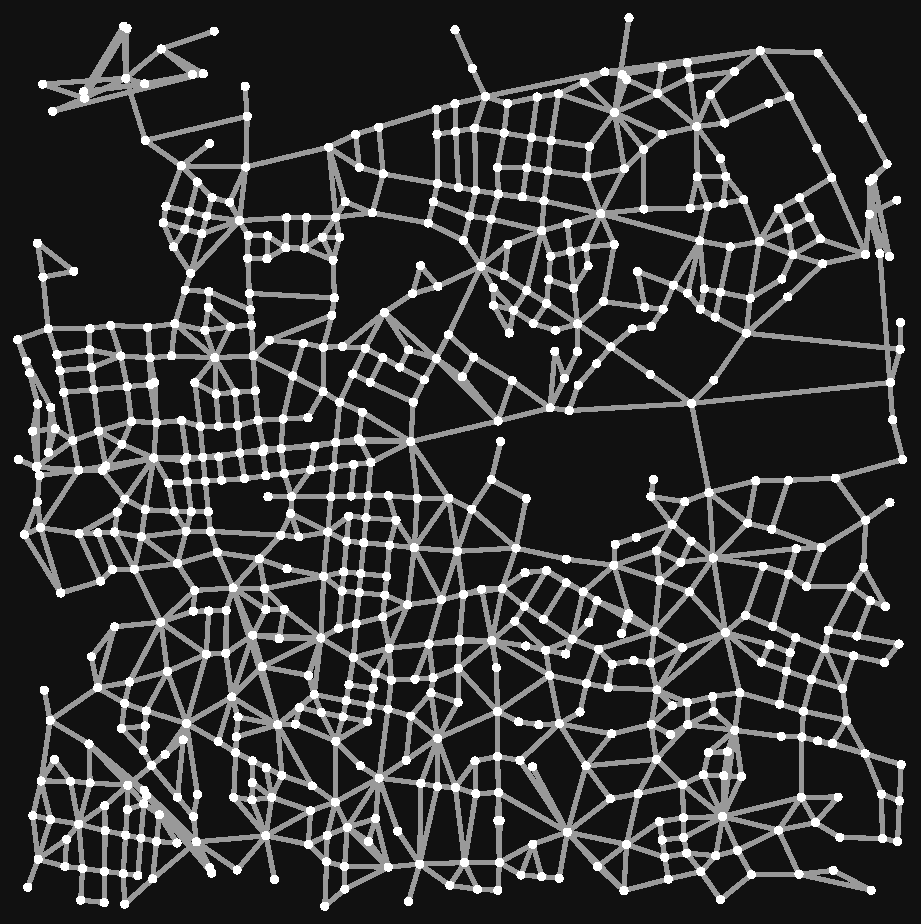
\includegraphics[width=.485\columnwidth]{graphics/tub.pdf}%
\hfill%
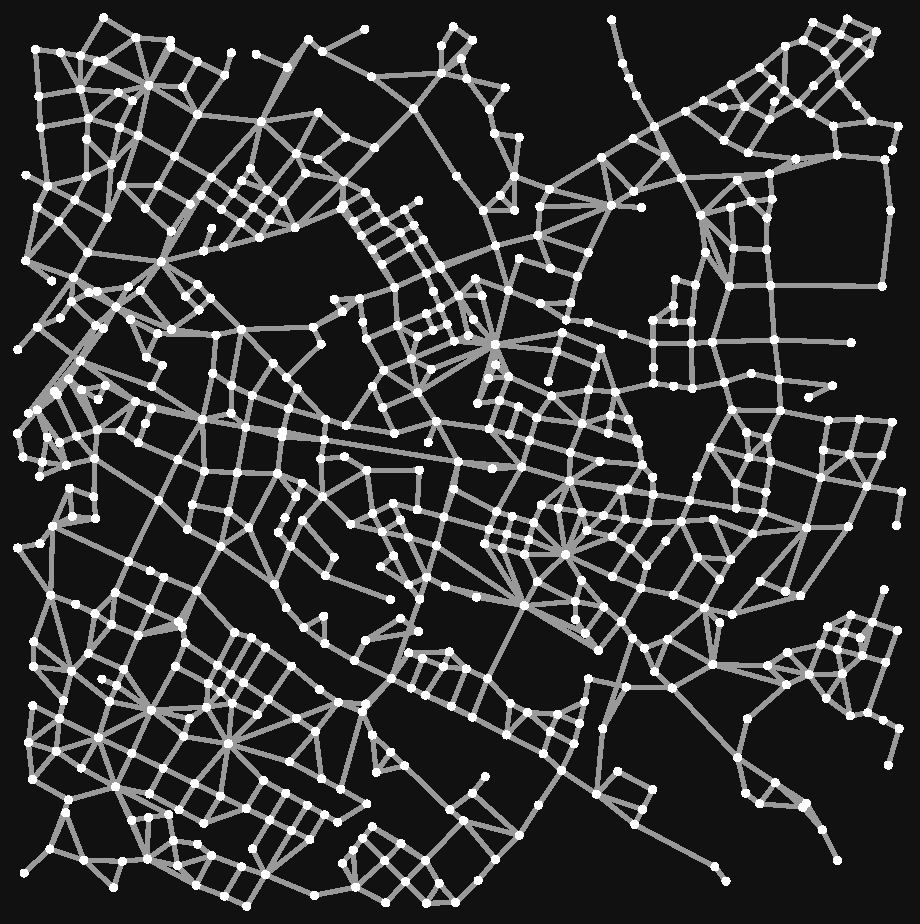
\includegraphics[width=.485\columnwidth]{graphics/ufrank.pdf}
\caption{Visualization of datasets created with OSMnx. left: tub, right: ufrank.
\osmattribute[Map data], see notes for more information}
\label{fig:datasets}
\end{figure}

\subsection{Similarity scoring}\label{subsec:similarity_scoring}

We use different similarity functions to score edges, some (like common neighbors, jaccard coefficient or adamic adar index)
have been used traditionally for link prediction~\cite[see][1021]{social_link_prediction}
while others are less commonly used.
In contrast to other applications for link prediction, road networks include spacial information
that will also be used for assigning similarity scores.

Let \(\Gamma(x)\) be the set of neighbors of a node \(x\) in a graph.
(One has \(\Gamma(x) = \{y \mid \{x, y\} \in E\}\) if \(E\) is the set of all edges in a graph.)
Let \(x, y\) be any two nodes in a graph.
\begin{description}
\item[common neighbors (CN)] the number of neighbors the two nodes share;
      \(|\Gamma(x) \cap \Gamma(y)|\)
\item[jaccard coefficient (JC)] a normalized coefficient denoting how many neighbors the two nodes share;\\
      \(\frac{|\Gamma(x) \cap \Gamma(y)|}{|\Gamma(x) \cup \Gamma(y)|}\)
\item[adamic adar index (AA)] a coefficient denoting how many neighbors the two nodes share with diminishing returns;
      \(\sum_{z \in \Gamma(x) \cap \Gamma(y)}\frac{1}{\log(\Gamma(z))}\)
\item[min. neighbors (min)] the number of neighbors of the node that has less neighbors\endnotemark;
      \(\min\{|\Gamma(x)|,|\Gamma(y)|\}\)
\item[max. neighbors (max)] the number of neighbors of the node that has more neighbors\addtocounter{endnote}{-1}\endnotemark;
      \(\max\{|\Gamma(x)|,|\Gamma(y)|\}\)
\item[geospacial x-distance (xdist)] the distance of the nodes' geographical locations regarding longitude only
\item[geospacial y-distance (ydist)] the distance of the nodes' geographical locations regarding latitude only
\item[geospacial distance (dist)] the euclidean distance of the nodes' geographical locations
\item[top-k shortest distance (short)] Introduced by \citeauthor{link_prediction_k_shortest}
      as a similarity function for link prediction,
      this is the sum of the lengths of the first \(k\) shortest paths between the nodes.~\cite{link_prediction_k_shortest}
      The authors found that small values for \(k\) worked best in their datasets~\cite[see][4]{link_prediction_k_shortest},
      so we chose a value of \(k = 3\).
      We also chose to consider the lengths of the shortest paths separately,
      so \textbf{short1} refers to the length of the shortest path,
      \textbf{short2} refers to the length of the shortest path excluding the first and
      \textbf{short3} refers to the length of the shortest path excluding the first two.
\end{description}
\endnotetext{As \autoref{subsec:road_networks_as_graphs} suggests,
the degree (number of neighbors) of a node contains information on the type of the node (intersection,  etc.)}

\section{Experiments}

The road networks described in \autoref{subsec:datasets} are split into a
test- and training-network by randomly assigning edges to either network.
We carry out our experiments with two different splits:
\begin{enumerate}
\item a 80-20 training-testing split (\textbf{tub20} and \textbf{ufrank20} respectively)
\item a 70-30 training-testing split (\textbf{tub30} and \textbf{ufrank30} respectively)
\end{enumerate}
Due to limited computing resources, we have run our experiment only five times
(for every dataset and splitting method) and the resulting values
referenced represent the mean over these five runs.

We apply the similarity functions described in \autoref{subsec:similarity_scoring}
to all non-existent connections of the training-network and evaluate the results using the test-network.

For every function we computed the \emph{area under the ROC-curve} (AUROC) and the results are shown in \autoref{tab:similarity_auroc}.
AUROC allows us to compare the performance of a function to random guessing~\cite[see][40]{informedness},
as guessing randomly for each datapoint would result in a AUROC-score of 0.5.\\
While calculating the AUROC-score it is assumed
that a higher similarity score corresponds to a higher probability of the link existing.
For some similarity functions this is not true, and instead the AUROC of their
negated output was computed, such that a lower similarity score leads to a higher link probability.
This has been highlighted in the referenced table with a \enquote{\n{}} before the abbreviation of the function.

\begin{table*}[tb]
\caption{AUROC for different similarity functions}
\label{tab:similarity_auroc}
\scriptsize
\renewcommand{\arraystretch}{0.8}
\resizebox{\linewidth}{!}{%
\begin{tabularx}{\textwidth}{lXXXXXXXXXXXX}
\toprule
&CN        &JC        &AA        &\n{}min   &\n{}max   &\n{}xdist
&\n{}ydist &\n{}dist  &\n{}short &\n{}short1&\n{}short2&\n{}short3\\
\midrule
% tub
\textbf{tub20} \hfill mean
&0.635504  &0.635623  &0.635659  &0.627206  &0.581656  &0.952672
&0.952200  &0.995198  &0.812849  &0.853254  &0.812823  &0.795867\\
\hfill std.
&0.013376  &0.013396  &0.013392  &0.008794  &0.018746  &0.001881
&0.001453  &0.000636  &0.033307  &0.027014  &0.031193  &0.032282\\
\midrule
\textbf{tub30} \hfill mean
&0.615754  &0.615837  &0.615859  &0.591949  &0.551532  &0.953862
&0.951671  &0.995839  &0.749292  &0.799927  &0.751449  &0.724398\\
\hfill std.
&0.010361  &0.010351  &0.010343  &0.005995  &0.007744  &0.001544
&0.001061  &0.000306  &0.013059  &0.012457  &0.012353  &0.012540\\
\midrule
% ufrank
\textbf{ufrank20} \hfill mean
&0.632681  &0.632904  &0.632783  &0.632304  &0.586775  &0.953170
&0.953767  &0.996590  &0.782483  &0.829498  &0.786609  &0.758246\\
\hfill std.
&0.013331  &0.013384  &0.013300  &0.014338  &0.015329  &0.001579
&0.001369  &0.000451  &0.024275  &0.026360  &0.025041  &0.020442\\
\midrule
\textbf{ufrank30} \hfill mean
&0.605373  &0.605493  &0.605448  &0.609986  &0.584332  &0.952126
&0.953461  &0.996258  &0.676313  &0.752542  &0.683670  &0.646840\\
\hfill std.
&0.004467  &0.004489  &0.004487  &0.008024  &0.014252  &0.000571
&0.000949  &0.000203  &0.038982  &0.034168  &0.039458  &0.035356\\
\bottomrule
\end{tabularx}
}
\end{table*}

The random forest classifiers have been trained on one complete dataset
and are being evaluated on the dataset they have not trained on.
A classifier trained on \enquote{tub20} and evaluated on \enquote{ufrank20} will be refered to as \enquote{tub20 on ufrank20}.
We have trained classifiers with 50 decision trees and a maximum tree depth of 10 (these have the suffix \enquote{small}),
and classifiers with 100 decision trees and a maximum depth of 50 (suffix \enquote{large}).
The results for some common performance metrics for classifiers are shown in \autoref{tab:classifier_metrics}.
Finally, we have also visualized the predictions of two of the trained classifiers in \autoref{fig:classifier_predictions} (these are not cherry-picked).

\begin{table}
\caption{Performance of the random forest classifiers}
\label{tab:classifier_metrics}
\scriptsize
\renewcommand{\arraystretch}{0.8}
\begin{tabularx}{\columnwidth}{@{}p{4em}@{\,}l@{\,}XXXXXX}
\toprule
&
&accuracy mean &accuracy std. &recall mean &recall std. &precision mean &precision std.\\
\midrule
\multirow{2}{=}{\textbf{tub20} on \textbf{ufrank20}}
&large
&0.998935      &0.000025      &0.189913    &0.018090    &0.530258       &0.033606\\
&small
&0.998945      &0.000023      &0.165929    &0.029215    &0.549297       &0.035229\\
\midrule
\multirow{2}{=}{\textbf{tub30} on \textbf{ufrank30}}
&large
&0.998412      &0.000032      &0.244223    &0.012845    &0.524902       &0.018915\\
&small
&0.998451      &0.000034      &0.235323    &0.017230    &0.556468       &0.023496\\
\midrule
\multirow{2}{=}{\textbf{ufrank20} on \textbf{tub20}}
&large
&0.998915      &0.000023      &0.237205    &0.025487    &0.551084       &0.021606\\
&small
&0.998925      &0.000031      &0.208588    &0.023491    &0.572757       &0.034146\\
\midrule
\multirow{2}{=}{\textbf{ufrank30} on \textbf{tub30}}
&large
&0.998410      &0.000027      &0.273833    &0.019809    &0.568415       &0.016990\\
&small
&0.998409      &0.000011      &0.244656    &0.018904    &0.576806       &0.007279\\
\bottomrule
\end{tabularx}
\end{table}

\begin{figure}[tb]
\centering
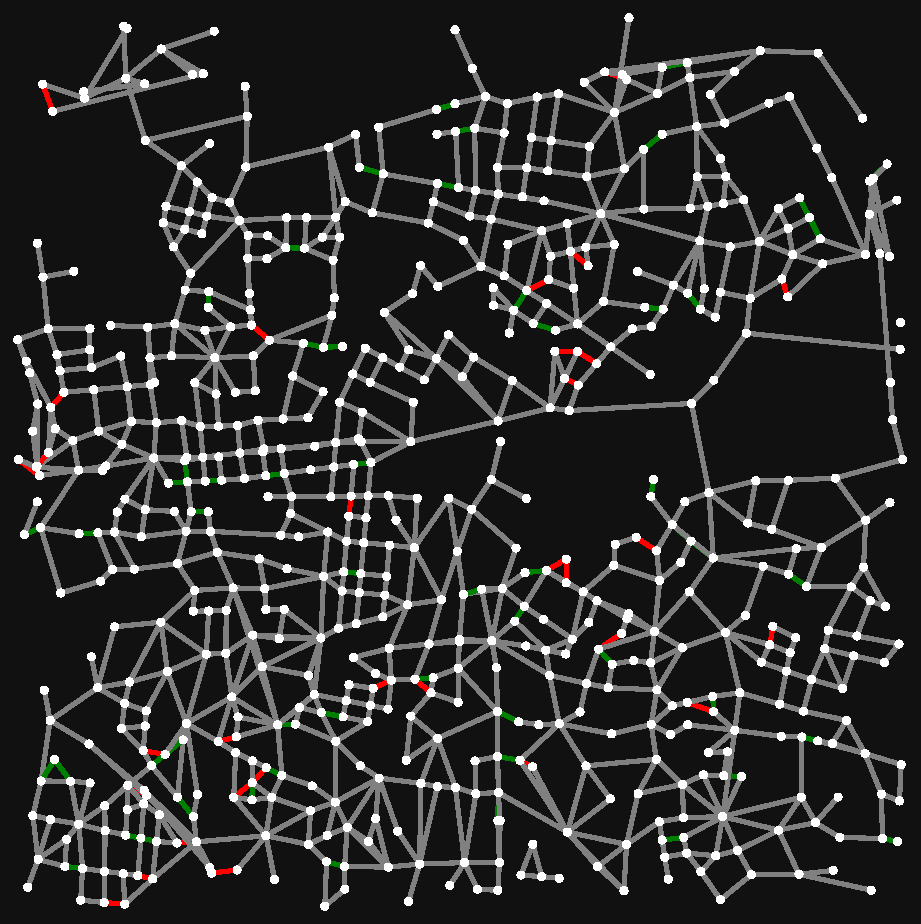
\includegraphics[width=.485\columnwidth]{graphics/tub_random_forest_classifier_cross_small.pdf}%
\hfill%
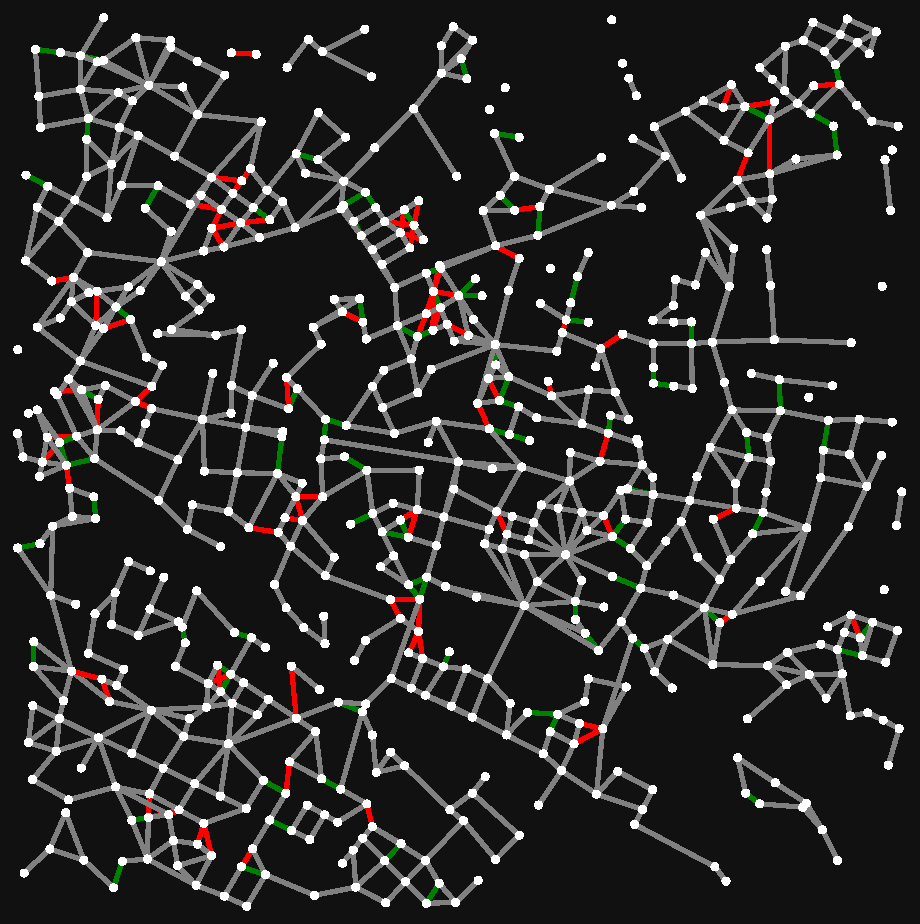
\includegraphics[width=.485\columnwidth]{graphics/ufrank_random_forest_classifier_cross_30_large.pdf}
\caption{Visualization of predictions created with OSMnx. left: ufrank20 on tub20 small, right: tub30 on ufrank30 large.
Grey edges are known (training-network), green edges represent correct guesses, red edges false ones; false negatives are not shown.
\osmattribute[Map data], see notes for more information}
\label{fig:classifier_predictions}
\end{figure}

\subsection{Discussion}

Our results show low AUROC for the similarity functions \enquote{CN}, \enquote{JC} and \enquote{AA},
confirming the findings of \citeauthor{road_link_prediction_subgraph}.~\cite[see][20]{road_link_prediction_subgraph}

In general the standard deviation is relatively low (speaking for the representativeness of the results)
and the similarity functions based on graph distance and on geospacial distance show the best performance.
However it should be noted, that computing the geographical distance was less time intensive.
Although not shown in the results above, calculating the function \enquote{short}
took on average over 400 \(\times\) more time than any other function in our computing environment.\\
Hence concerning datasets we used or datasets similar to these,
geospacial distance can be considered as an important similarity function.

While there are trends between different datasets and splits,
they lie within the standard-deviation.
Since only the results of five experiments are being considered,
we will abstain from making any conclusions from these trends.

\section{Conclusion}\label{sec:conclusion}

In this paper we presented a method for predicting links using different similarity metrics and random tree classifiers.
Although we have run only few experiments,
on our datasets our method shows a useful recall-rate of over 16\% on average while maintaining an acceptable precision of over 52\%.

Our method however does not
\begin{itemize}
\item consider obstacles in the terrain, such as buildings or lakes,
\item consider multiple roads/connections between nodes,
\item produce the shape of roads or location of nodes
\end{itemize}
and has not been tested with data from possible real-world applications or rural areas.

Future work should not only focus on these limitations,
but should also explore other methods of prediction on the specific domain of road networks to improve performance
and test the feasibility for the real-world applications mentioned in the introduction of this paper.

Nevertheless, our paper introduced geospacial distance as a important feature to consider for link prediction in road networks and
proposed a method for dataset extraction that can be applied to any real-world location using publicly available data.
Finally given the performance of our classifiers, we show link prediction
on road networks is feasible and thus we believe link prediction on road networks can have a interesting future.

\addtoendnotes{\textbf{The maps presented in this paper contain information from OpenStreetMap (\url{openstreetmap.org}), which is made available
here under the Open Database License (ODbL) (\url{http://opendatacommons.org/licenses/odbl/1.0/}).}}

\theendnotes

\printbibliography

\end{document}
